\section{Parallel program profiler analysis}
After the parallel program implementation, another round of profiling using \code{cProfile} was conducted. This was done on the initial testing laptop,
with 4 workers, on the same dataset as the first round of profiling. The results from the main process that orchestrates the other processes and aggregates their results can be
found in \ref{fig:parallel_profiler_main}. The results from two of the workers can be found in figure \ref{fig:parallel_profiler_w1} and figure \ref{fig:parallel_profiler_w2}.

For the main process, it is apparent that \code{post\_process\_parallel}, the function that makes the trade ID:s unique after the parallel worker processes have finished
executing, adds non-negligible overhead. \code{aggregate\_result} contains the code that creates the other processes and waits for these to produce their partial results,
aggregating them as they are produced. This code takes up 84\% of the total time, while the remaining 16\% of the code is effectively overhead.
In addtion, as mentioned in section \ref{section:sequential_profiler} as a possibility, \code{\_prepare} is called for each
worker process, resulting in extra overhead. It is conceivable that these sources of overhead are less noticable when processing a larger dataset, as the effects of
the functions that are called only one time take up a smaller amount of the total running time if the dataset contains a larger number of rows.

For the worker processes, the results are similar to the results from profiling the sequential program in section \ref{section:sequential_profiler}, but with lower
\code{cumtime} values. This is expected due to the lower number of rows per worker. The same functions as in the sequential program are responsible for the largest
portion of the running time, \code{process\_record}, \code{post\_process\_record}, \code{consume\_record}, and \code{\_prepare}.

\begin{figure}[ht]
  \lstinputlisting[basicstyle=\tiny]{figures/profiling_parallel_19_may_main.txt}
  \caption{Main process in parallel program \code{cProfile} output}
  \label{fig:parallel_profiler_main}
\end{figure}
\clearpage

\begin{figure}[ht]
  \lstinputlisting[basicstyle=\tiny]{figures/profiling_parallel_19_may_31147.txt}
  \caption{Worker 1 in parallel program \code{cProfile} output}
  \label{fig:parallel_profiler_w1}
\end{figure}
\clearpage

\begin{figure}[ht]
  \lstinputlisting[basicstyle=\tiny]{figures/profiling_parallel_19_may_31148.txt}
  \caption{Worker 2 in parallel program \code{cProfile} output}
  \label{fig:parallel_profiler_w2}
\end{figure}
\clearpage

\section{Transformation benchmarks}
The benchmarks for the experiments are outlined below. For each dataset, the results consist of a table containing
speedup, real time, user time, system time, and memory usage for each worker number. The standard deviation is represented
as a value following the $\pm$ sign. The value S in worker column signifies the original sequential program, while 1 is the
parallel program with a single worker. In addition to the tables, the real time, speedup, and memory usage are illustrated
using plots in order to visually demonstrate how the values change with the number of workers. In the plots for real time
and memory usage, the standard deviation is illustrated using black bars above and below each data point\footnote{
The standard deviation is shown for all plots of real time and memory usage, but it may be too small to be seen for some of the plots.}.

\section{Benchmark tables}
\subsection{Tiny}
The benchmark for the tiny dataset can be found in figure \ref{fig:dataset_1_table}.
The table displays the number of workers, the speedup (sequential run real time divided by real time), real time,
user time, system time, and memory usage. The standard deviation is displayed with a value following the $\pm$ sign.

\begin{figure}[ht]
\centering
\resizebox{\linewidth}{!}{%
\begin{tabular}{|c|c|c|c|c|c|}%
  \hline
  \bfseries Workers & \bfseries Speedup & \bfseries Real (s) & \bfseries User (s) & \bfseries System (s) & \bfseries Memory usage (MB)
  \csvreader[respect all,head to column names]{figures/dataset_1/dataset_1_table.csv}{workers=\w,speedup=\spd,real=\r,user=\u,system=\s,memory_usage_mb=\m}
  {\\\hline \w & \spd & \r & \u & \s & \m}
  \\ \hline
\end{tabular}}
\caption[Tiny dataset benchmark table.]{Tiny dataset benchmark table. The table displays the number of workers, the speedup (sequential run real time divided by real time), real time,
user time, system time, and memory usage. The standard deviation is displayed with a value following the $\pm$ sign.}
\label{fig:dataset_1_table}
\end{figure}

\subsection{Small}
The benchmark for the small dataset can be found in figure \ref{fig:dataset_2_table}.
The table displays the number of workers, the speedup (sequential run real time divided by real time), real time,
user time, system time, and memory usage. The standard deviation is displayed with a value following the $\pm$ sign.

\begin{figure}[ht]
\centering
\resizebox{\linewidth}{!}{%
\begin{tabular}{|c|c|c|c|c|c|}%
  \hline
  \bfseries Workers & \bfseries Speedup & \bfseries Real (s) & \bfseries User (s) & \bfseries System (s) & \bfseries Memory usage (MB)
  \csvreader[respect all,head to column names]{figures/dataset_2/dataset_2_table.csv}{workers=\w,speedup=\spd,real=\r,user=\u,system=\s,memory_usage_mb=\m}
  {\\\hline \w & \spd & \r & \u & \s & \m}
  \\ \hline
\end{tabular}}
\caption[Small dataset benchmark table.]{Small dataset benchmark table. The table displays the number of workers, the speedup (sequential run real time divided by real time), real time,
user time, system time, and memory usage. The standard deviation is displayed with a value following the $\pm$ sign.}
\label{fig:dataset_2_table}
\end{figure}

\subsection{Medium}
The benchmark for the medium dataset can be found in figure \ref{fig:dataset_3_table}.
The table displays the number of workers, the speedup (sequential run real time divided by real time), real time,
user time, system time, and memory usage. The standard deviation is displayed with a value following the $\pm$ sign.

\begin{figure}[ht]
\centering
\resizebox{\linewidth}{!}{%
\begin{tabular}{|c|c|c|c|c|c|}%
  \hline
  \bfseries Workers & \bfseries Speedup & \bfseries Real (s) & \bfseries User (s) & \bfseries System (s) & \bfseries Memory usage (MB)
  \csvreader[respect all,head to column names]{figures/dataset_3/dataset_3_table.csv}{workers=\w,speedup=\spd,real=\r,user=\u,system=\s,memory_usage_mb=\m}
  {\\\hline \w & \spd & \r & \u & \s & \m}
  \\ \hline
\end{tabular}}
\caption[Medium dataset benchmark table.]{Medium dataset benchmark table. The table displays the number of workers, the speedup (sequential run real time divided by real time), real time,
user time, system time, and memory usage. The standard deviation is displayed with a value following the $\pm$ sign.}
\label{fig:dataset_3_table}
\end{figure}

\subsection{Large}
The benchmark for the small dataset can be found in figure \ref{fig:dataset_4_table}.
The table displays the number of workers, the speedup (sequential run real time divided by real time), real time,
user time, system time, and memory usage. The standard deviation is displayed with a value following the $\pm$ sign.

\begin{figure}[ht]
\centering
\resizebox{\linewidth}{!}{%
\begin{tabular}{|c|c|c|c|c|c|}%
  \hline
  \bfseries Workers & \bfseries Speedup & \bfseries Real (s) & \bfseries User (s) & \bfseries System (s) & \bfseries Memory usage (MB)
  \csvreader[respect all,head to column names]{figures/dataset_4/dataset_4_table.csv}{workers=\w,speedup=\spd,real=\r,user=\u,system=\s,memory_usage_mb=\m}
  {\\\hline \w & \spd & \r & \u & \s & \m}
  \\ \hline
\end{tabular}}
\caption[Large dataset benchmark table.]{Large dataset benchmark table. The table displays the number of workers, the speedup (sequential run real time divided by real time), real time,
user time, system time, and memory usage. The standard deviation is displayed with a value following the $\pm$ sign.}
\label{fig:dataset_4_table}
\end{figure}

\section{Execution time}

\subsection{Tiny}
The real execution time for the tiny dataset can be found in figure \ref{fig:dataset_1_real_time}.
The X axis shows the number of workers, where 0 signifies the sequential program run.
The Y axis shows the real execution time for each worker value. The standard deviation is displayed with black bars around each data point. Real time
increases as number of workers increase. The data points at 10 and 13 workers show high standard deviation.
\begin{figure}[ht]
  \centering
  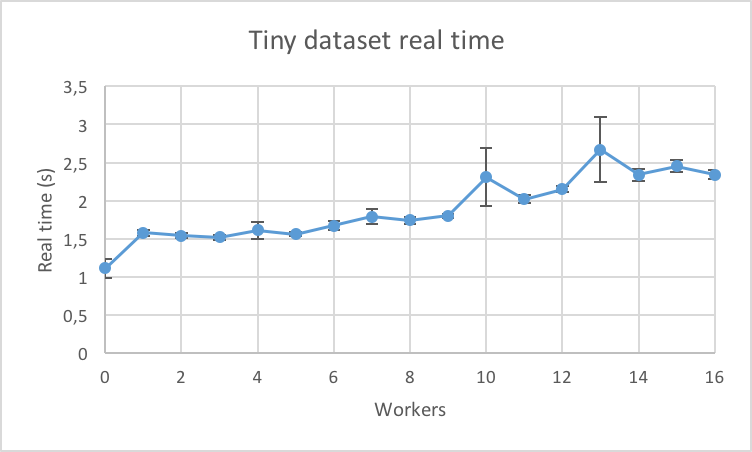
\includegraphics[width=120mm]{figures/dataset_1/dataset_1_real_time.png}
  \caption[Real time plot for the tiny dataset.]{Real time plot for the tiny dataset. The X axis shows the number of workers, where 0 signifies the sequential program run.
  The Y axis shows the real execution time for each worker value. The standard deviation is displayed with black bars around each data point. Real time
  increases as number of workers increase. The data points at 10 and 13 workers show high standard deviation.}
  \label{fig:dataset_1_real_time}
\end{figure}

\subsection{Small}
The real execution time for the small dataset can be found in figure \ref{fig:dataset_2_real_time}.
The X axis shows the number of workers, where 0 signifies the sequential program run.
The Y axis shows the real execution time for each worker value. The standard deviation is displayed with black bars around each data point. The real time
decreases with each added worker up to 8 workers, where it evens out. The decrease in real time for each added worker becomes smaller as the number increases.
\begin{figure}[ht]
  \centering
  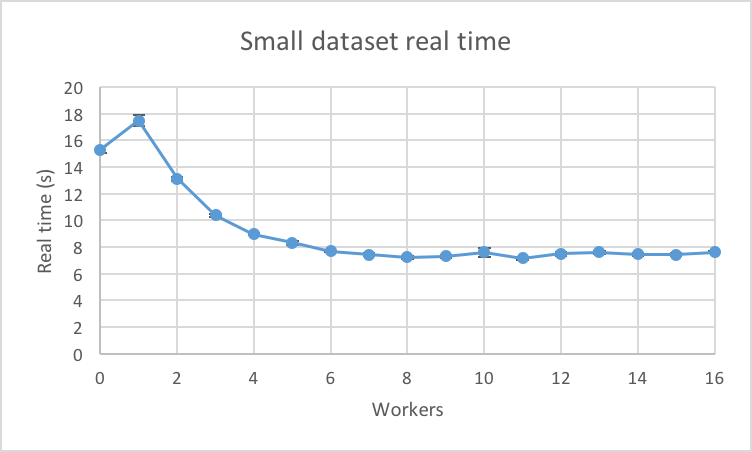
\includegraphics[width=120mm]{figures/dataset_2/dataset_2_real_time.png}
  \caption[Real time plot for the small dataset.]{Real time plot for the small dataset. The X axis shows the number of workers, where 0 signifies the sequential program run.
  The Y axis shows the real execution time for each worker value. The standard deviation is displayed with black bars around each data point. The real time
  decreases with each added worker up to 8 workers, where it evens out. The decrease in real time for each added worker becomes smaller as the number increases.}
  \label{fig:dataset_2_real_time}
\end{figure}

\subsection{Medium}
The real execution time for the medium dataset can be found in figure \ref{fig:dataset_3_real_time}.
The X axis shows the number of workers, where 0 signifies the sequential program run.
The Y axis shows the real execution time for each worker value. The standard deviation is displayed with black bars around each data point. The real time
decreases with each added worker up to 8 workers, where it evens out. The decrease in real time for each added worker becomes smaller as the number increases.
\begin{figure}[ht]
  \centering
  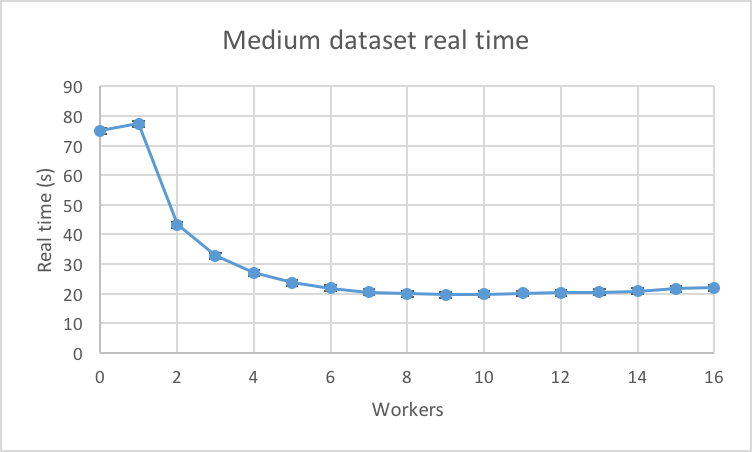
\includegraphics[width=120mm]{figures/dataset_3/dataset_3_real_time.png}
  \caption[Real time plot for the medium dataset.]{Real time plot for the medium dataset. The X axis shows the number of workers, where 0 signifies the sequential program run.
  The Y axis shows the real execution time for each worker value. The standard deviation is displayed with black bars around each data point. The real time
  decreases with each added worker up to 8 workers, where it evens out. The decrease in real time for each added worker becomes smaller as the number increases.}
  \label{fig:dataset_3_real_time}
\end{figure}

\subsection{Large}
The real execution time for the small dataset can be found in figure \ref{fig:dataset_4_real_time}.
The X axis shows the number of workers, where 0 signifies the sequential program run.
The Y axis shows the real execution time for each worker value. The standard deviation is displayed with black bars around each data point. The real time
decreases with each added worker up to 12 workers, where it evens out. The decrease in real time for each added worker becomes smaller as the number increases.
\begin{figure}[ht]
  \centering
  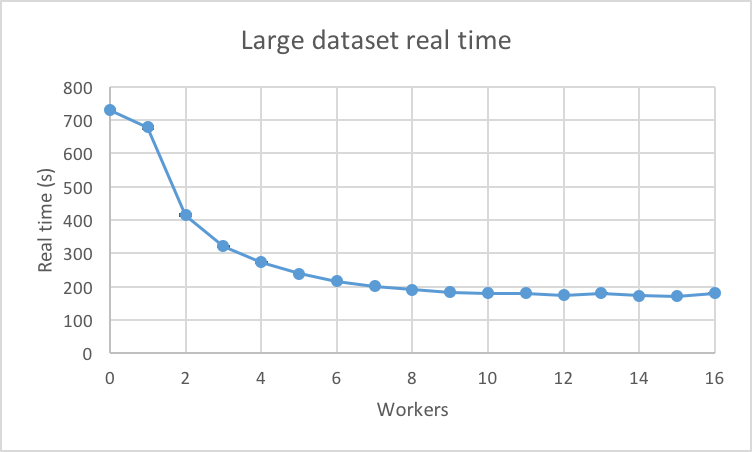
\includegraphics[width=120mm]{figures/dataset_4/dataset_4_real_time.png}
  \caption[Real time plot for the large dataset.]{Real time plot for the large dataset. The X axis shows the number of workers, where 0 signifies the sequential program run.
  The Y axis shows the real execution time for each worker value. The standard deviation is displayed with black bars around each data point. The real time
  decreases with each added worker up to 12 workers, where it evens out. The decrease in real time for each added worker becomes smaller as the number increases.}
  \label{fig:dataset_4_real_time}
\end{figure}

\section{Speedup}

\subsection{Tiny}
The speedup for the tiny dataset can be found in figure \ref{fig:dataset_1_speedup}.
The X axis shows the number of workers, and the Y axis shows a scalar value signifying the speedup as
``number of times faster than sequential execution''. Speedup decreases with each added worker, down to about half the speed of the sequential execution.
\begin{figure}[ht]
  \centering
  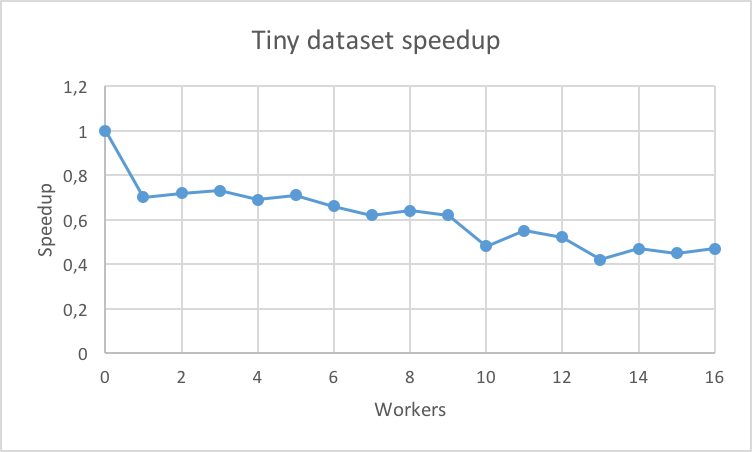
\includegraphics[width=120mm]{figures/dataset_1/dataset_1_speedup.png}
  \caption[Speedup plot for tiny dataset.]{Speedup plot for the tiny dataset. The X axis shows the number of workers, and the Y axis shows a scalar value signifying the speedup as
  ``number of times faster than sequential execution''. Speedup decreases with each added worker, down to about half the speed of the sequential execution.}
  \label{fig:dataset_1_speedup}
\end{figure}

\subsection{Small}
The speedup for the small dataset can be found in figure \ref{fig:dataset_2_speedup}.
The X axis shows the number of workers, and the Y axis shows a scalar value signifying the speedup as
``number of times faster than sequential execution''. Speedup increases with each worker, evening out around 8 workers and 2.1X speedup.
\begin{figure}[ht]
  \centering
  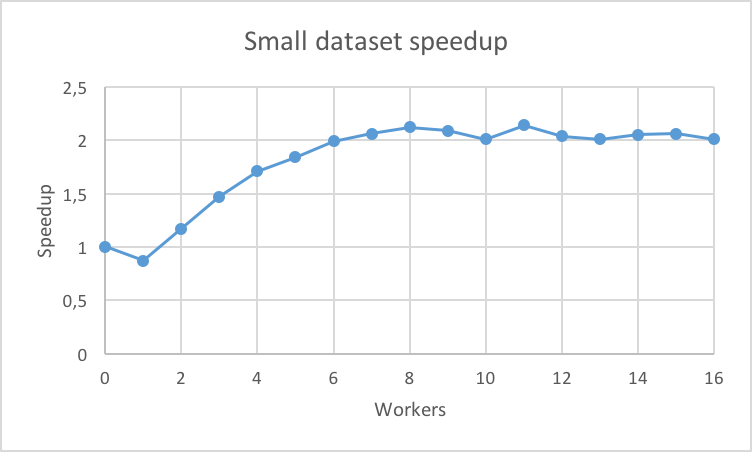
\includegraphics[width=120mm]{figures/dataset_2/dataset_2_speedup.png}
  \caption[Speedup plot for the small dataset.]{Speedup plot for the small dataset. The X axis shows the number of workers, and the Y axis shows a scalar value signifying the speedup as
  ``number of times faster than sequential execution''. Speedup increases with each worker, evening out around 8 workers and 2.1X speedup.}
  \label{fig:dataset_2_speedup}
\end{figure}

\subsection{Medium}
The speedup for the medium dataset can be found in figure \ref{fig:dataset_3_speedup}.
The X axis shows the number of workers, and the Y axis shows a scalar value signifying the speedup as
``number of times faster than sequential execution''. Speedup increases with each worker, evening out around 8-9 workers and 3.8X speedup.
\begin{figure}[ht]
  \centering
  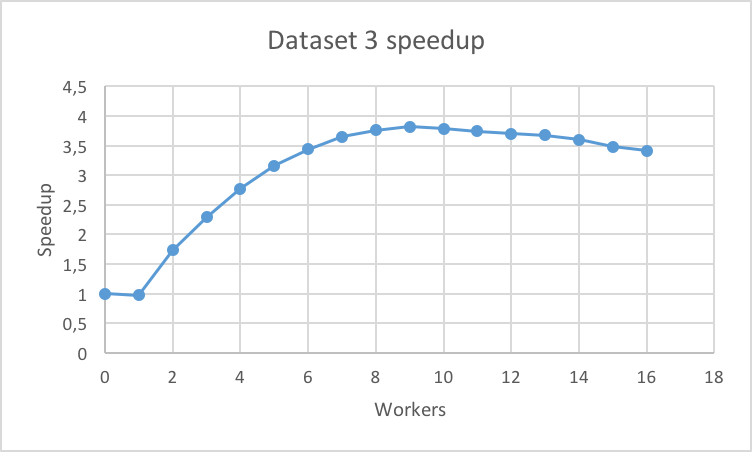
\includegraphics[width=120mm]{figures/dataset_3/dataset_3_speedup.png}
  \caption[Speedup plot for the medium dataset.]{Speedup plot for the medium dataset. The X axis shows the number of workers, and the Y axis shows a scalar value signifying the speedup as
  ``number of times faster than sequential execution''. Speedup increases with each worker, evening out around 8-9 workers and 3.8X speedup.}
  \label{fig:dataset_3_speedup}
\end{figure}

\subsection{Large}
The speedup for the large dataset can be found in figure \ref{fig:dataset_4_speedup}.
The X axis shows the number of workers, and the Y axis shows a scalar value signifying the speedup as
``number of times faster than sequential execution''. Speedup increases with each worker, evening out around 12 workers and 4.2X speedup.
\begin{figure}[ht]
  \centering
  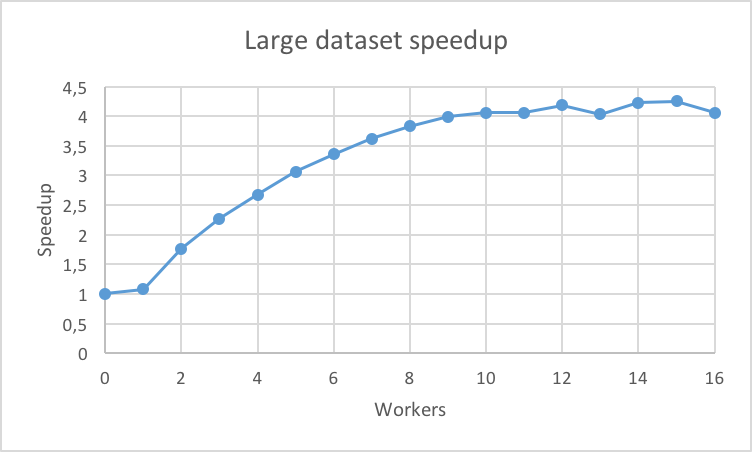
\includegraphics[width=120mm]{figures/dataset_4/dataset_4_speedup.png}
  \caption[Speedup plot for the large dataset.]{Speedup plot for the large dataset. The X axis shows the number of workers, and the Y axis shows a scalar value signifying the speedup as
  ``number of times faster than sequential execution''. Speedup increases with each worker, evening out around 12 workers and 4.2X speedup.}
  \label{fig:dataset_4_speedup}
\end{figure}

\section{Memory consumption}

\subsection{Tiny}
The memory consumption for the tiny dataset can be found in figure \ref{fig:dataset_1_memory}.
The X axis shows the numner of workers, and the Y axis shows the total memory usage as
a sum of the highest memory usage for each worker process, in addition to the main process. Memory usage increases close to linearly with each added worker,
up to about 1.6 GB for 16 workers.
\begin{figure}[ht]
  \centering
  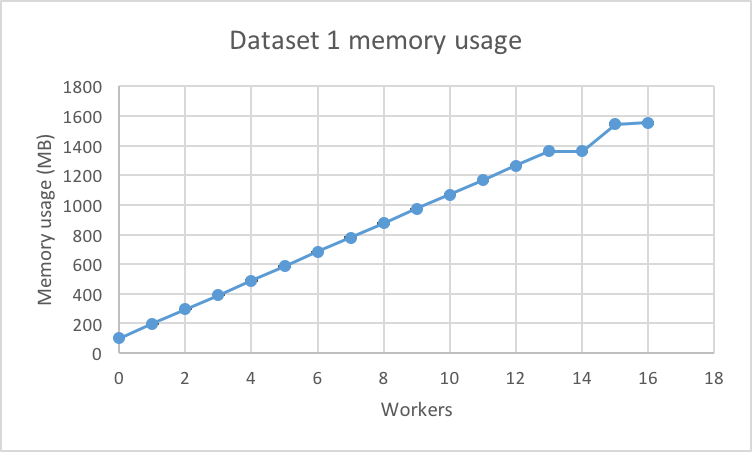
\includegraphics[width=120mm]{figures/dataset_1/dataset_1_memory.png}
  \caption[Memory usage plot for the tiny dataset.]{Memory usage plot for the tiny dataset. The X axis shows the numner of workers, and the Y axis shows the total memory usage as
  a sum of the highest memory usage for each worker process, in addition to the main process. Memory usage increases close to linearly with each added worker,
  up to about 1.6 GB for 16 workers.}
  \label{fig:dataset_1_memory}
\end{figure}

\subsection{Small}
The memory consumption for the tiny dataset can be found in figure \ref{fig:dataset_2_memory}.
The X axis shows the numner of workers, and the Y axis shows the total memory usage as
a sum of the highest memory usage for each worker process, in addition to the main process. Memory usage increases close to linearly with each added worker,
up to about 2 GB for 16 workers.
\begin{figure}[ht]
  \centering
  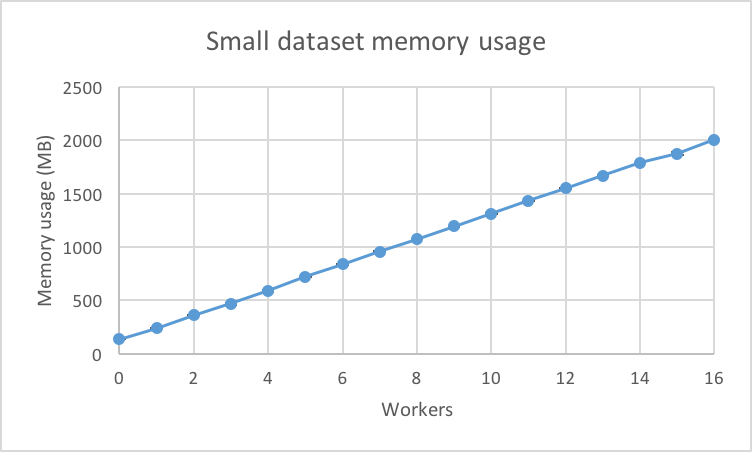
\includegraphics[width=120mm]{figures/dataset_2/dataset_2_memory.png}
  \caption[Memory usage plot for the small dataset.]{Memory usage plot for the small dataset. The X axis shows the numner of workers, and the Y axis shows the total memory usage as
  a sum of the highest memory usage for each worker process, in addition to the main process. Memory usage increases close to linearly with each added worker,
  up to about 2 GB for 16 workers.}
  \label{fig:dataset_2_memory}
\end{figure}

\subsection{Medium}
The memory consumption for the tiny dataset can be found in figure \ref{fig:dataset_3_memory}.
The X axis shows the numner of workers, and the Y axis shows the total memory usage as
a sum of the highest memory usage for each worker process, in addition to the main process. Memory usage increases close to linearly with each added worker,
up to about 6 GB for 16 workers.
\begin{figure}[ht]
  \centering
  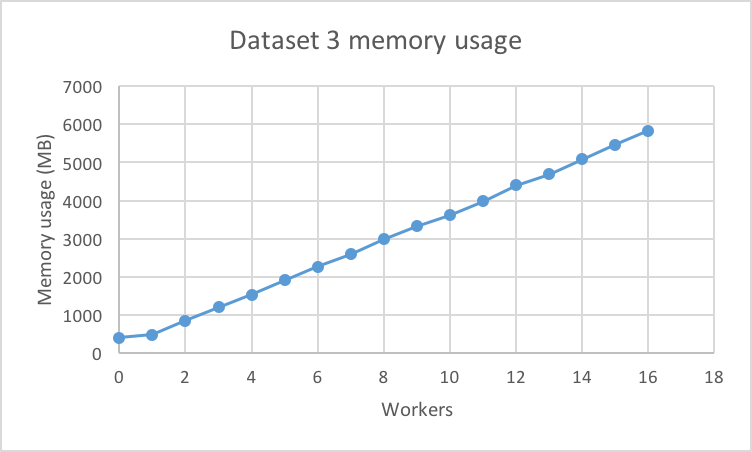
\includegraphics[width=120mm]{figures/dataset_3/dataset_3_memory.png}
  \caption[Memory usage plot for the medium dataset.]{Memory usage plot for the medium dataset. The X axis shows the numner of workers, and the Y axis shows the total memory usage as
  a sum of the highest memory usage for each worker process, in addition to the main process. Memory usage increases close to linearly with each added worker,
  up to about 6 GB for 16 workers.}
  \label{fig:dataset_3_memory}
\end{figure}

\subsection{Large}
The memory consumption for the tiny dataset can be found in figure \ref{fig:dataset_4_memory}.
The X axis shows the numner of workers, and the Y axis shows the total memory usage as
a sum of the highest memory usage for each worker process, in addition to the main process. Memory usage increases close to linearly with each added worker,
up to about 8.8 GB for 16 workers.
\begin{figure}[ht]
  \centering
  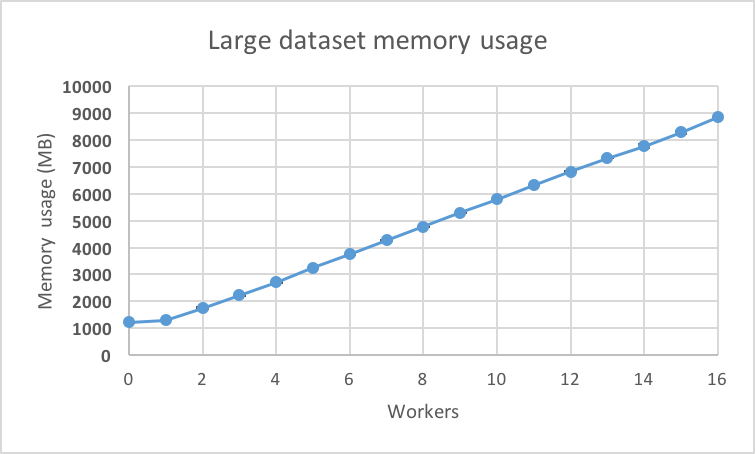
\includegraphics[width=120mm]{figures/dataset_4/dataset_4_memory.png}
  \caption[Memory usage plot for the large dataset.]{Memory usage plot for the large dataset. The X axis shows the numner of workers, and the Y axis shows the total memory usage as
  a sum of the highest memory usage for each worker process, in addition to the main process. Memory usage increases close to linearly with each added worker,
  up to about 8.8 GB for 16 workers.}
  \label{fig:dataset_4_memory}
\end{figure}

